In section \ref{section:2.2.1} maintainability was defined as how understandable, repairable, and extendable a software system is. To ensure such properties, it is important to know software engineering concepts such as complexity, cohesion and coupling. Because measuring these properties proved to determine the effort of maintainability \cite{33}.

IEEE defines software complexity as “the degree to which a system or component has a design or implementation that is difficult to understand and verify \cite{20}. Complexity makes it harder to understand a class; therefore, it gets harder to maintain \cite{59}. Software complexity prevents interactions between different modules, increases the chance of introducing bugs when making changes, thus decreasing maintainability. High coupling and lack of cohesion stand out as the main causes of complexity in software systems. Fig. \ref{fig:maintainability_factors} shows the relationship between maintainability, complexity, cohesion and coupling.

\begin{figure}[ht!]
    \centering
    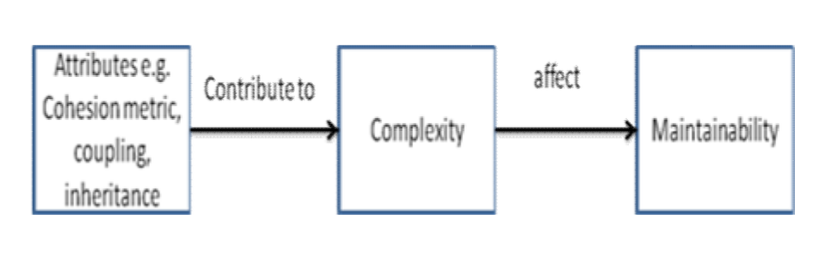
\includegraphics[scale=0.6]{figures/maintainability_factors.png}
    \caption{Relationship between cohesion, coupling, complexity and maintainability \protect\cite{33}}
    \label{fig:maintainability_factors}
\end{figure}
 
Coupling defines the interdependency between the classes. Changes done in one class affects the dependant classes. Software systems with high coupling are hard to maintain. Cohesion is the degree of the relation and interdependency of the members of the class. It promotes software maintainability because high cohesive classes are more understandable, maintainable and easy to modify.
Complexity, cohesion and coupling are in a tight relationship among themselves, and they all directly affect software maintainability \cite{33}. 

